%===================================== CHAP 3 =================================

\chapter{Experimental} \label{chapter3}
This chapter will introduce the experimental samples that will be investigated by computational models. It will begin by introducing the various nano tools used in the works of Brakstad \cite{brakstad_thesis} and \cite{gasbcones} in fabricating and characterizing the samples, before ... . The nanostructures introduced in this chapter will be modelled with a finite element method approach via the commercial FEM software COMSOL Multiphysics.
\section{Quick notes regarding nano tools}
\text{\color{red}fjern seksjon?}
\begin{itemize}
    \item FIB
    \item SEM
    \item e-beam evaporation
\end{itemize}

%%%%%%%%%%%%%%%%%%%%%%%%%%%%%%%%%%%%%%%%%%%%%%%%%%%%%%%%%%

%%%%%%%%%%%%%%%%%%%%%%%%%%%%%
\section{Hemispheroidal gold particles on SiO$_2$ substrate}
\begin{itemize}
    \item introduce samples. AFM/SEM pictures. over-etching. Total height of gold particles and the assumed mound is found to be 40nm[?] by studying AFM data [ref til figur hvis brukt i ch2] in the open-source software Gwyddion[ref].
    \item Problems with previous model
    \item Achievement goals   
    \item Why are these type of nanostructures interesting? Evt ha kun i Introduction
\end{itemize}

In the thesis works of Brakstad \cite{brakstad_thesis}, several 3-material nanostructures were manufactured consisting of Au-nanoparticles on a flat SiO$_2$ substrate in air. The substrates were covered with a thin gold film by an e-beam evaporator\footnote{Electron beam physical vapor deposition; a vacuum deposition method used to produce thin films and coatings. An electron beam evaporates atoms from a target anode under high vacuum, causing everything in the vacuum chamber to be coated with a thin layer of the anode material.} before the nanostructures were milled out with focused ion beam microscopy. \unsure{elaborate?} The nanostructures appeared as Au hemispheroids distributed in a square or rectangular pattern on a glass surface, see figure \ref{fig:ch3_AuSiO2_sketch+SEM}. Three chosen structures from this work will henceforth be discussed, known as sample 6, sample 5A and sample 5B. The deposited Au film thickness before milling were initially 40nm (samples 5A and 5B) and 20nm (sample 6). These samples were characterized by scanning electron microscopy (SEM) images and MM ellipsometer measurements \cite{brakstad_thesis}, while samples 5A and 6 were further discussed in detail by M. Kildemo et al. \cite{Brakstad:15}\cite{Kildemo2017}. The ellipsometric measurements done in \cite{brakstad_thesis} were performed with a RC2 ellipsometer provided by J.A. Woollam Co., which detects wavelengths from 210 nm (5.9 eV) to 1700 nm (0.73 eV). In addition, full azimuthal rotational measurements (varying $\phi_0$) were done for a given AOI, $\theta_0$, in order to identify symmetries caused by any anisotropic geometries in the fabricated samples. For all samples there was found next to zero depolarization. They were also shown to exhibit rich optical responses supporting LSPRs\cite{brakstad_thesis}. 

\begin{figure}[htb]
    \begin{subfigure}{0.3\textwidth}
        \centering
        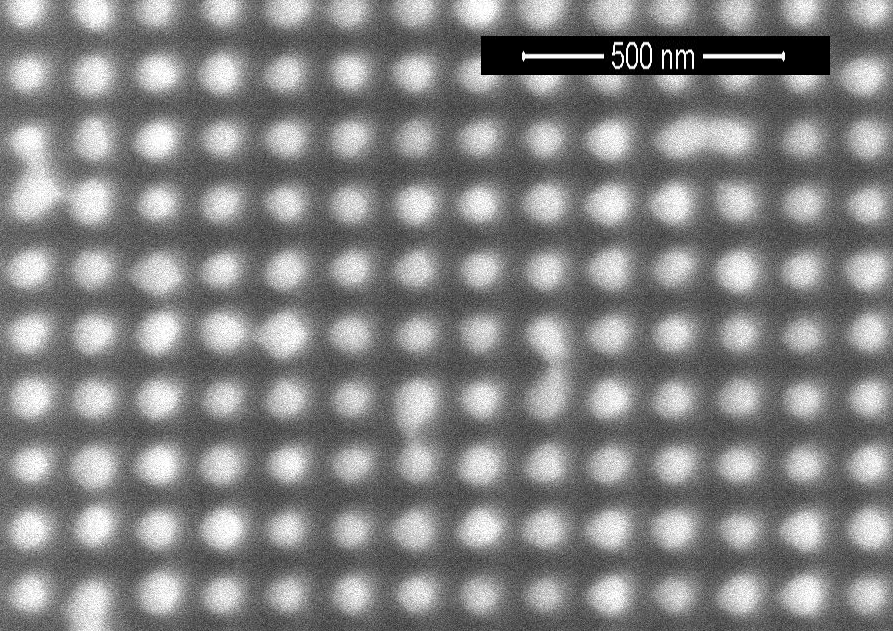
\includegraphics[width=\linewidth]{figures/Ch3/S6_SEM.png}
        \caption{}
        \label{fig:ch3_S6_SEM}
    \end{subfigure}
    \begin{subfigure}{0.3\textwidth}
        \centering
        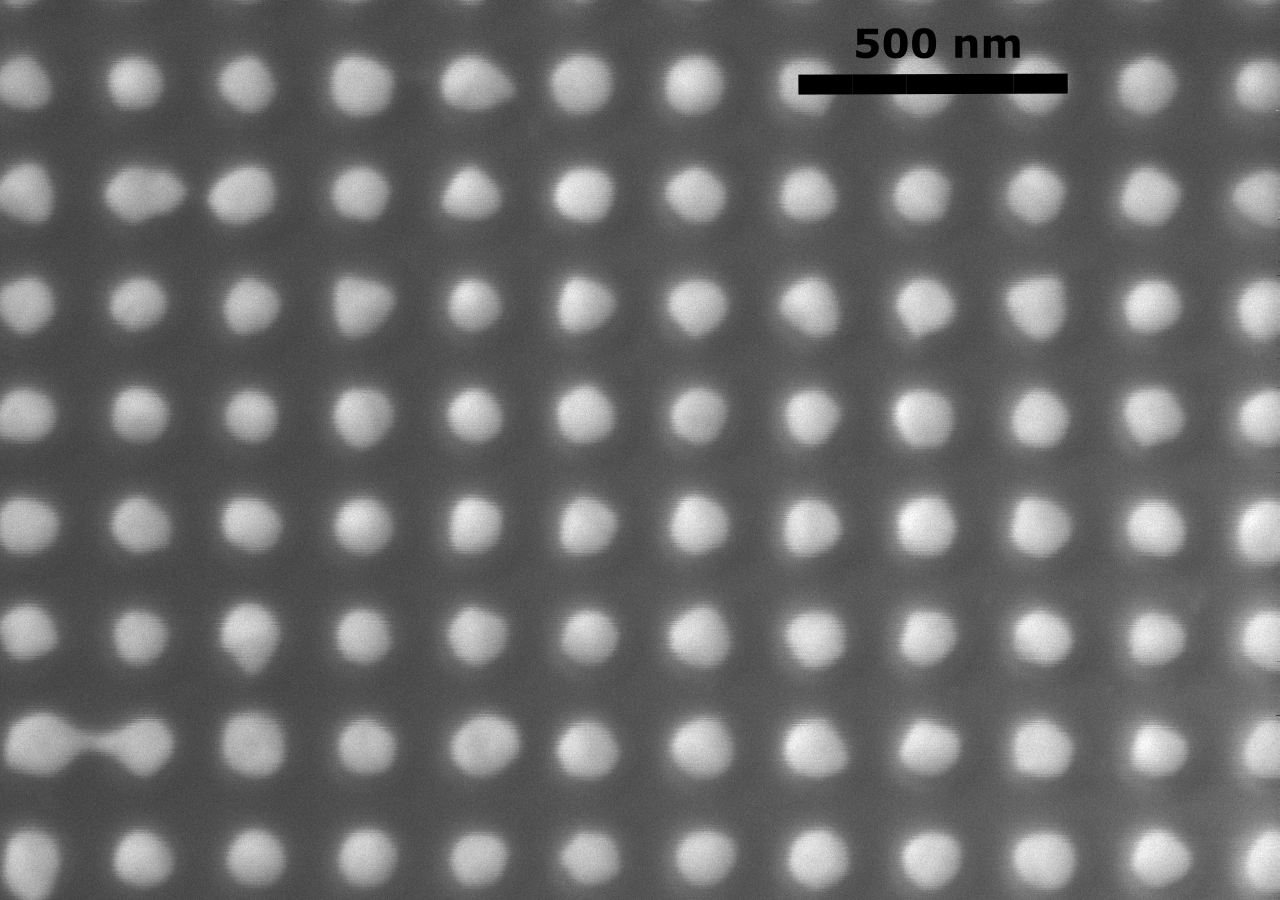
\includegraphics[width=\linewidth]{figures/Ch3/S5A_SEM.png}
        \caption{}
        \label{fig:ch3_S5A_SEM}
    \end{subfigure}
    \begin{subfigure}{0.3\textwidth}
        \centering
        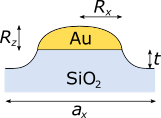
\includegraphics[width=\linewidth]{figures/Ch3/goldhemispheroids_sketch.png}
        \caption{}
        \label{fig:ch3_AuSiO2_sketch}
    \end{subfigure}
    \caption{SEM images of (a) sample 6 and (b) sample 5A. (c) Cross-section in xz-plane of the unit cell setup of the gold hemispheroidal particles on a glass substrate. \color{red}gjør (c) svart-hvit}
    \label{fig:ch3_AuSiO2_sketch+SEM}
\end{figure}

An unintended effect of the milling process caused an over-etching into the substrate of several nanometers, suggesting that each Au particle on all the samples lies on top of a dielectric mound, as sketched in figure \ref{fig:ch3_AuSiO2_sketch} (however, the exact shape of the mound can only be speculated). This can also be observed by close inspection of figure \ref{fig:ch3_S5A_SEM}, where a vague mound geometry can be made out surrounding each particle. The geometry of all three samples are characterized by their lattice constants $a_{x,y}$, Au particle radii $R_{x,y,z}$ and the thickness $t$ of the SiO$_2$ mound as depicted in figure \ref{fig:ch3_AuSiO2_sketch}.

\subsection{Sample 6}
Sample 6 was originally made to fabricate small dots close to the quasi-static approximation arranged in a square array. A SEM image of the sample can be found in figure \ref{fig:ch3_S6_SEM}. After the milling, the particles were found to be hemispheroids with lateral radius $R_{xy} = 38$nm and lattice constant $a_{xy} = 125$nm, see figure \ref{fig:ch3_AuSiO2_sketch}. Through a combination of atomic-force microscopy (AFM) and SEM images, the total height of particle and mound was found to be 40nm. Separating particle height $R_z$ and mound height $t$ individually was however more difficult to estimate. Under the assumption that the other parameter estimations were accurate, a parameter sweep of $R_z$ and $t$ was performed in the COMSOL model of sample 6. The set of parameters with a resulting LSPR resonance closest resembling that of the experimental results were chosen, see appendix \ref{appendix:sample_parameters}. This concluded in $R_z=32$nm and $t=8$nm, however, the uncertainty associated with the height profiling must be emphasized.

\subsection{Sample 5A}
Sample 5A was originally created as one in a series of similar nanostructures to investigate the how the distance between the Au spheres influence the LSP resonance energy. The GranFilm software\footnote{\url{http://web.phys.ntnu.no/~ingves/Software/GranFilm/}} was used to estimate the sample 5A parameters\footnote{Simulations performed by PhD. student Jean-Philippe Banon at the Department of Physics, NTNU.}, see appendix \text{\color{red}ref}. The experimental data sets were fitted with respect to the morphological parameters of the sample ($R_x$, $R_y$, $R_z$, $a_x$, $a_y$) using GranFilm\cite{Kildemo2017}. The sample was found to be less uniform than originally intended, the lattice being slightly rectangular and the Au particle slightly elliptic in the lateral direction while lying on top of a large mound, see table \ref{tab:GoldLatticeParameters}. 

\subsection{Sample 5B}
\label{sec:ch3_sample5B}
Sample 5B is a biaxial anisotropic system due to the high eccentricity of the Au particles and rectangular lattice, as seen in figure \ref{fig:S5B_schematic_overview}. This was done by making ellipses of the 40 nm Au film. The sample was found to have little re-deposition and exhibit relatively stable geometric shape\cite{brakstad_thesis}. It was created for the purpose of observing how different dielectric functions in each of the three spatial directions would present itself in the ellipsometric data. 

\begin{figure}
    \begin{subfigure}{0.5\textwidth}
        \centering
        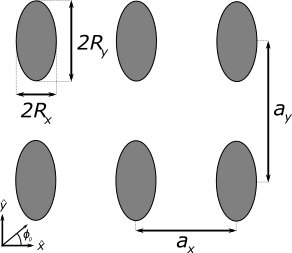
\includegraphics[width=\linewidth]{figures/Ch3/s5b/S5B_topview_phi.png}
        \caption{}
        \label{fig:S5B_schematic_overview_topview}
    \end{subfigure}
    \begin{subfigure}{0.5\textwidth}
        \centering
        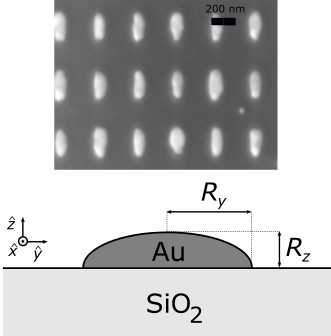
\includegraphics[width=0.83\linewidth]{figures/Ch3/s5b/S5B_sideview+SEM.png}
        \caption{}
        \label{fig:S5B_schematic_overview_SEM_sideview}
    \end{subfigure}
    \caption{(a) Top view schematic of sample 5B. Azimuthal angle of the incident beam $\phi_0$ is defined along positive x-direction. (b) Above: SEM image of sample 5B. Below: schematic side view of the sample when neglecting the mound.}
    \label{fig:S5B_schematic_overview}
\end{figure}

The same GranFilm optimization process was done for sample 5B parameters as for sample 5A. A mound thickness of around 15 nm \text{\color{red} 20?} was found by studying the total height profile from AFM images and subtracting particle height $R_z$ found from the parameter fitting procedure. An indication of a dielectric mound can also be observed around each Au particle by close inspection of figure \ref{fig:S5B_schematic_overview_SEM_sideview}. However, due to limitations in computer power, sample 5B was simulated with no mound (i.e. flat substrate) as the amount of finite elements to solve when having a fine mesh detailing the mound geometry in such a large unit cell system were beyond the scope of the desktop computer used for the simulations. 

\text{\color{red}skal denne seksjonen \emph{kun} ha experimentell info,} 

\text{\color{red}eller er det greit å skyte inn info om modelleringa her?}

The geometric parameters that ended up being used in COMSOL simulations for the three samples are summarized in table \ref{tab:GoldLatticeParameters}. 





\begin{table}[h!]
\centering
\caption{Parameters (given in nanometers) for different samples of gold hemispheroidal particles defined by the radii $R_x$, $R_y$ and $R_z$ over a SiO2 substrate, evenly distributed on a grid defined by lattice constants $a_x$ and $a_y$. Each particle lies on top of a SiO2 mound of height $t$, except sample 5B which lies on a flat substrate.}
\label{tab:GoldLatticeParameters}
\begin{tabular}{l l l l}
            &   Sample 6    &   Sample 5A   &   Sample 5B   \\
    \hline 
    $a_x$   &   125       &   207.2         &   315.4            \\
    $a_y$   &   125       &   209.9         &   443.9            \\
    $R_x$   &   38        &   60.3          &   47.4            \\
    $R_y$   &   38        &   61.3          &   113.2            \\
    $R_z$   &   32        &   34.8          &   34.4            \\
    $t$     &   8         &   36.9          &   0            \\
    \hline
\end{tabular}
\end{table}




%%%%%%%%%%%%%%%%%%%%%%%%%%%%%
\section{Tilted GaSb cones}
Ion beam sputtering of flat surfaces can in some circumstances lead to spontaneous formation of nanoscale patterns, a phenomena which could open alternative ways of controlling the surface roughness of functional materials\cite{Nerbo_insituFormationGasb}. A distinct type of pattern formation was found for sputtering on certain semiconductors, like GaSb. These materials form pillar patterns and GaSb is considered to be the most conspicuous example\cite{Nerbo_insituFormationGasb}.

In the works of \cite{gasbcones}, densely packed GaSb nanocones are self-assembled using low energy Ion Beam Sputtering, which involves ejecting mono-crystalline GaSb from a targeting source onto a substrate, where the growth is driven by the difference in diffusion velocity and sputtering yield of the two components of the semiconductor. A misalignment of the ion gun caused a slight tilt of the cones, which were originally intended to be directed normal to the substrate surface\cite{gasbcones}. Ellipsometric characterization of such structures are particularly practical since shadowing effects render atomic force microscopy non-applicable\cite{Nerbo_inclinedGasb}.

Spectroscopic Mueller Matrix Ellipsometry gives access to anisotropic electronic characteristics of the material, where an anisotropic Bruggeman effective medium model was applied to model the spectroscopic data. The anisotropic Bruggeman model is essentially a generalization of equation (\ref{eq:EMA_Bruggeman}) for ellipsoidal inclusion by applying the polarizability of an ellipsoid (\ref{eq:polarizability_ellipsoid}). Through mathematical models, parameters like the tilt of the cones and relative diameters and average height of the cones are found\cite{gasbcones}. Average cone separation was found using another non-destructive technique called Grazing-Incidence Small-Angle X-ray Scattering (GISAXS) where surface sensitivity is obtained by using a grazing incident angle of X-rays. GISAXS was also used to confirm film anisotropy induced by the nanopillar tilt\cite{gasbcones}. These sample parameters are summarized in table \ref{tab:gasbparameters} while figure \ref{fig:GaSbConeGeometry} visualizes the cone geometry.

%\unsure{IsGISAXS og MME er komplementære for å finne ut parametrene. Dvs hvis du først begynner å snakke om MM ellipsometri ble brukt til å finne D1,D2,h, tiltvinkel, burde du også forklare hvordan de finner d? }
\begin{table}[h]
\centering
\caption{Parameter values for tilted cones of GaSb as found in \cite{gasbcones}.}
\label{tab:gasbparameters}
\begin{tabular}{l l}
    \hline 
    $h$         &   39 nm    \\
    $\theta$    &   4.8$^\circ$   \\
    $D_1$       &   $d$    \\
    $D_2$       &   0.04$d$    \\
    $d$         &   40 nm   \\
    $\beta$     &   64^$$\circ$ \\
    \hline
\end{tabular}
\end{table}


The main motivation of modeling these tilted GaSb cones is to attempt a continuation of the COMSOL model for other periodic nanostructures than the gold hemispheroids on glass substrate, which the model initially will be tailored for. The nanocones differ greatly from the other samples in both size and shape, and the dense cone distribution should not be represented by a square lattice. The secondary objective is to attempt a high energy simulation up to $24$ eV to model the response the ellipsometer and the anisotropic Bruggeman model\footnote{The EMA is limited to structures sufficiently smaller than the wavelength of light, i.e. the electric field is assumed to be constant over an inclusion in the mixed material so that the phase of the wave is approximately the same over the size of the inclusion. Models taking into account retardation effects must be applied for smaller wavelengths.} is unable to capture. AFM analysis found the cones to be distributed with six nearest neighbours, which allows an assumption of a hexagonal lattice\cite{gasbcones}. 

\begin{figure}
    \centering
    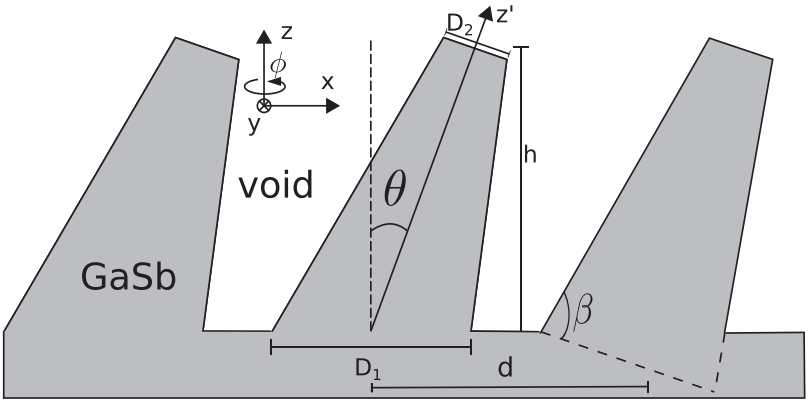
\includegraphics[scale=0.33]{figures/Ch3/GaSbConesGeometry.png}
    \caption{Tilt angle $\theta$ of the GaSb nanocones, the height $h$, the bottom and top diameters $D_1$ and $D_2$, the average distance to nearest neighbour $d$, and base angle $\beta$. Sketch taken from \cite{gasbcones}.}    
    \label{fig:GaSbConeGeometry}
\end{figure}




\clearpage